\documentclass{article}
\usepackage{tikz}
\usetikzlibrary{hobby}

\begin{document}

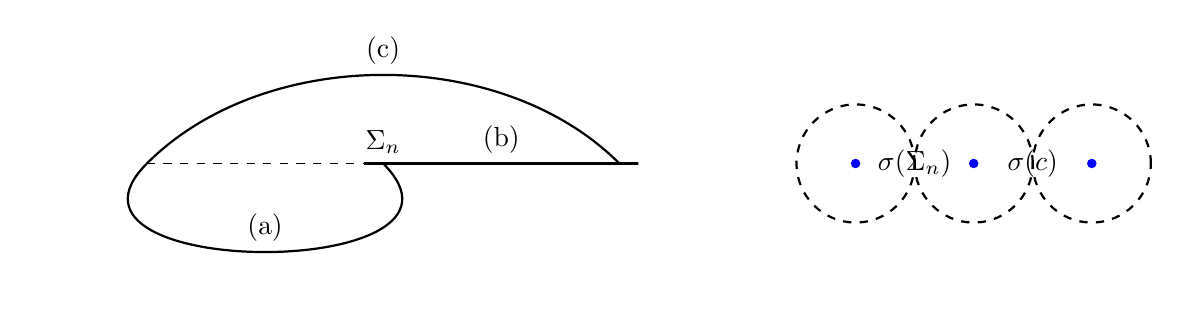
\begin{tikzpicture}[scale=1.5]
    % Define coordinates for the shapes
    \coordinate (A) at (-2,0);
    \coordinate (B) at (0,0);
    \coordinate (C) at (2,0);
    
    % Draw the main shapes
    \draw[thick] (A) .. controls +(-1,-1) and +(1,-1) .. (B) node[pos=0.5,above] {(a)};
    \draw[thick] (B) .. controls +(-1,0) and +(1,0) .. (C) node[pos=0.5,above] {(b)};
    \draw[thick] (C) .. controls +(-1,1) and +(1,1) .. (A) node[pos=0.5,above] {(c)};
    
    % Draw the dashed line
    \draw[dashed] (A) -- (C) node[midway,above] {$\Sigma_n$};
    
    % Draw the transformed shapes
    \draw[thick,dashed] (4,0) circle (0.5);
    \draw[thick,dashed] (5,0) circle (0.5);
    \draw[thick,dashed] (6,0) circle (0.5);
    
    % Label the transformed shapes
    \node at (4.5,0) {$\sigma(\Sigma_n)$};
    \node at (5.5,0) {$\sigma(c)$};
    
    % Add points on the circles
    \filldraw[blue] (4,0) circle (1pt);
    \filldraw[blue] (5,0) circle (1pt);
    \filldraw[blue] (6,0) circle (1pt);
\end{tikzpicture}

\end{document}